\chapter{Spécifications et Analyse des besoins}
Nous nous sommes intéressés au Top 10 d'Owasp qui nous a servi de cahiers de charge pour notre recueil de besoins. Les spécifications ont été faites sur la base de ce document. La version originale du document est disponible en annexe.\\
Le Top 10 Owasp, en recensant les dix risques de sécurite les plus critiques des applications Web, les explique et donne pour chacune de celles-ci, un ensemble de directives de codage à mettre en œuvre pour se protéger de ces risques de sécurite. Cependant, le document original n'est pas assez parlant pour bon nombre de personnes et le fait qu'il soit rédigé en anglais est un obstacle pour d'autres. Nous avons tenté d'expliquer chaque point du Top 10 afin de les faire connaître aux développeurs. Cela a fait l'objet d'un document distribué aux développeurs et affiché dans les locaux de HubSo. De même, nous avons, pour chaque risque, recensé les pratiques à mettre en œuvre pour s'en prémunir. Celles-ci feront l'objet des specifications et de l'analyse.

\section{Spécifications}

\subsection{Spécifications fonctionnelles}
Les spécifications fonctionnelles décrivent les processus métier dans lesquels notre système devra intervenir, les tâches prises en charge par le système. Dans notre cas, il s'agira des tâches préconisées par le Top 10 pour chacune des risques de sécurite. 

\subsubsection{Les Acteurs}
Un acteur représente un rôle joué par une entité externe (utilisateur humain, dispositif matériel
ou autre système) qui interagit directement avec le système étudié.\\
Notre système est principalement en interaction avec les autres applications utilisant les différentes fonctionnalités mises à disposition par celui-ci. 

\subsubsection{Les fonctionnalités générales}
Notre système met à la disposition des applications qui l'utilisent un ensemble de fonctionnalités leur permettant de gérer les différentes risques de sécurite énoncées par le Top 10. Ces fonctionnalités, sont dans un premier regroupées en modules, chaque module correspondant à la gestion d'un risque.

\textbf{\RIGHTarrow Gestion des injections}\\
Ce module regroupe les fonctions de sécurité permettant de se protéger des injections. Pour prévenir les injections, les fonctions de sécurités suivantes doivent être mises à disposition par le système : \\
- la validation des entrées ; \\
- l’encodage des données ; \\
- le paramétrage de requêtes ;
- le cryptage de données avec un algorithme fort.\\

\textbf{\RIGHTarrow Gestion des violations de Gestion d’Authentification}\\
Ce module regroupe les fonctions de sécurité permettant de se protéger des violations de gestion d'authentification. Pour prévenir la violation de gestion d'authentification, les fonctions de sécurités suivantes doivent être disponibles dans notre système : \\
- l'authentification ;\\
- la déconnexion ;\\
- la vérification de la force d'un mot de passe ; \\
- la génération de mots de passe forts ; \\ 
- la génération d'ids de session ; \\
- la génération de tokens anti-csrf [WX] ; \\
- la journalisation des événements de connexion (logging) ; \\
- le cryptage de données avec un algorithme fort.\\

\textbf{\RIGHTarrow Gestion des expositions de données sensibles}\\
Ce module regroupe les fonctions de sécurité permettant d'éviter l'exposition de données sensibles. Pour ce faire, les fonctions de sécurités suivantes doivent être disponibles dans notre système : \\
- le hachage fort de mots de passe avec un sel\footnote{donnée ajoutée au mot de passe avant hachage} ; \\
- le paramétrage des entêtes HTTP (Entête Cache essentiellement) ; \\
- le cryptage de données avec un algorithme fort.\\

\textbf{\RIGHTarrow Gestion des attaques sur les entités XML externes}\\
Ce module regroupe les fonctions de sécurité permettant de se protéger des attaques sur les entités XML externes. Il contient les fonctions de sécurités : \\
- l'encodage de données en HTML ; \\
- la validation des entrées.\\

\textbf{\RIGHTarrow Gestion des violations de contrôle d’accès}\\
Ce module regroupe les fonctions de sécurité permettant de se protéger des violations de contrôle d'accès. Pour prévenir les violations de contrôle d'accès, les fonctions de sécurités suivantes doivent être mises à disposition par le système : \\
- la vérification des autorisations sur les ressources (autorisations sur les fichiers, urls, fonctions) ; \\
- la vérification des rôles des utilisateurs ; \\
- l'authentification ; \\
- la déconnexion ; \\
- la journalisation des accès aux ressources et évènements de connexion.\\

\textbf{\RIGHTarrow Gestion des mauvaises configurations de sécurité}\\
Ce module regroupe les fonctions de sécurité permettant d'éviter les problèmes de sécurité découlant des mauvaises configurations de sécurité. On a principalement : \\
- le paramétrage des entêtes HTTP : il s'agit de toutes les entêtes HTTP relatives à la sécurité (Entêtes HSTS, X-Frame-Options, X-XSS-Protection, X-Content-Type-Options, CSP, X-Permitted-Cross-Domain-Policies entre autres). \\


\textbf{\RIGHTarrow Gestion des cross-site scripting (XSS)}\\
Ce module regroupe un ensemble de fonctions de sécurité permettant de se protéger des attaques XSS. Il s'agit de : \\
- la validation des entrées ;\\
- la sanitization des entrées ;\\
- l'encodage des sorties selon le contexte de sortie (HTML, CSS, JavaScript)\footnote{Toute donnée devant être ajoutée au code source}; \\
- le paramétrage des entêtes HTTP (CSP principalement).\\

%\textbf{\RIGHTarrow Gestion des désérialisations non sécurisée}\\


\textbf{\RIGHTarrow Gestion de l'utilisation de composants vulnérables}\\
Ce module regroupe les fonctions de sécurité relatives à l'utilisation de composants vulnérables. Il regroupe les fonctionnalités suivantes : \\
- la détection de composants vulnérables ; \\
- la notification de nouvelle version d'un composant.\\

\textbf{\RIGHTarrow Gestion de la journalisation et de la surveillance insuffisante}\\
Ce module regroupe les fonctions de sécurité relatives à la journalisation et à la surveillance. Il s'agit de journaliser afin d'avoir une trace de ce qui se passe dans le système mais aussi surveiller afin d'être réactif par rapport aux évènements du système. Les fonctionnalités sont les suivantes :\\
- la journalisation des évènements. \\


\subsection{Spécifications non fonctionnelles}
Les besoins non fonctionnelles ou exigences techniques portent sur les différents points suivants :
- le pinning de certificats ; \\
- l'utilisation de protocoles sécurisés; \\
- The preferred option is to use a safe API, which avoids the The preferred option is to use a safe API, which avoids the The preferred option is to use a safe API, which avoids use of the interpreter entirely or provides a parameterized interface or migrate to use Object Relational Mapping Tools (ORMs).\\
- Do not ship or deploy with any default credentials, particularly for admin users.\\
- Implement weak-password checks, such as testing new or changed passwords against a list of the top 10000 worst passwords.\\
- etablir une politique de mots de passe; \\
- A repeatable hardening process that makes it fast and easy to deploy another environment that is properly locked down. Development, QA, and production environments should all be configured identically, with different credentials used in each environment. This process should be automated to minimize the effort required to setup a new secure environment ;
- A minimal platform without any unnecessary features, components, documentation, and samples. - Remove or do not install unused features and frameworks.
- A task to review and update the configurations appropriate to all security notes, updates and patches as part of the patch management process (see A9:2017-Using Components with Known Vulnerabilities). In particular, review cloud storage permissions (e.g. S3 bucket permissions). \\
- A segmented application architecture that provides effective, secure separation between components or tenants, with segmentation, containerization, or cloud security groups (ACLs).
- Sending security directives to clients, e.g. Security Headers.
- An automated process to verify the effectiveness of the configurations and settings in all environments.\\
- portabilité \\
- compatibilité\\
- formation\\
- efficacité : efficacité en temps, efficacité en ressources\\
- facilité d'intégration\\
- Toute information confidentielle fournie par les  clients via l’Internet sera cryptée avec le système XYZ  ou par l’algorithme, la méthode....ABC..  \\
- Tous les logiciels du côté client vont être  téléchargés et installés à partir du navigateur, sans que  le poste du client ne soit redémarré ou configuré manuellement \\
- Le comportement du programme doit être paramétrable par des fichiers texte de configuration \\
%\textbf{\RIGHTarrow Gestion des mauvaises configurations de sécurité}\\
%\textbf{\RIGHTarrow Gestion des désérialisations non sécurisée}\\
- autres besoins non fonctionnels specifies par les autres points;


\section{Analyse}
Après avoir défini les acteurs et énuméré les fonctionnalités générales du système, nous passons à la phase d'analyse. Nous utiliserons les diagrammes de cas d'utilisation pour mieux représenter ce qui est attendu du système. Pour certains cas d'utilisation, une description textuelle sera faite. Nous utiliserons aussi des diagrammes d'activité pour illustrer le séquencement des actions par rapport à certains cas d'utilisation.\\
Pour des besoins de concision, chaque point du Top 10 sera considéré comme un package et comportera les fonctionnalités définies plus tôt. Ces packages sont les suivants : \\
- package gestion des injections\\
- package gestion des violations de Gestion d’Authentification\\
- package gestion des expositions de données sensibles\\
- package gestion des attaques sur les entités XML externes\\
- package gestion des violations de contrôle d’accès\\
- package gestion des cross-site scripting (XSS)\\
- package gestion de l'utilisation de composants vulnérables\\
- package gestion de la journalisation et de la surveillance insuffisante\\
La figure \ref{fig:8.1} ci-dessous reprèsente ces différents packages.
\begin{figure}[h!]
	\centering
	\begin{minipage}{18cm}
		\centering
		{\includegraphics[height=0.27\textheight]{fig/Package-Diagram.png}}
	\end{minipage}
	\caption{Diagramme de packages du système}
	\label{fig:8.1}
\end{figure}
Et, étant donné que certaines pratiques recommandées pour un risque, peuvent aussi l'être pour d'autres, nous présenterons à la volée, dans un deuxième temps, toutes les fonctionnalités attendues par les applications pour se protéger au moins des dix risques de sécurite présentes dans le Top 10.\\

\subsection{Package Gestion des injections}

\subsubsection{Diagramme de cas d'utilisation}
Le diagramme de cas d'utilisation du package "Gestion des injections" est representé ci-dessous. Il comprend les cas d'utilisation permettant à une application donnée de mitiger les risques d'injection.\\ 
\begin{figure}[h!]
	\centering
	\begin{minipage}{12cm}
		\centering
		{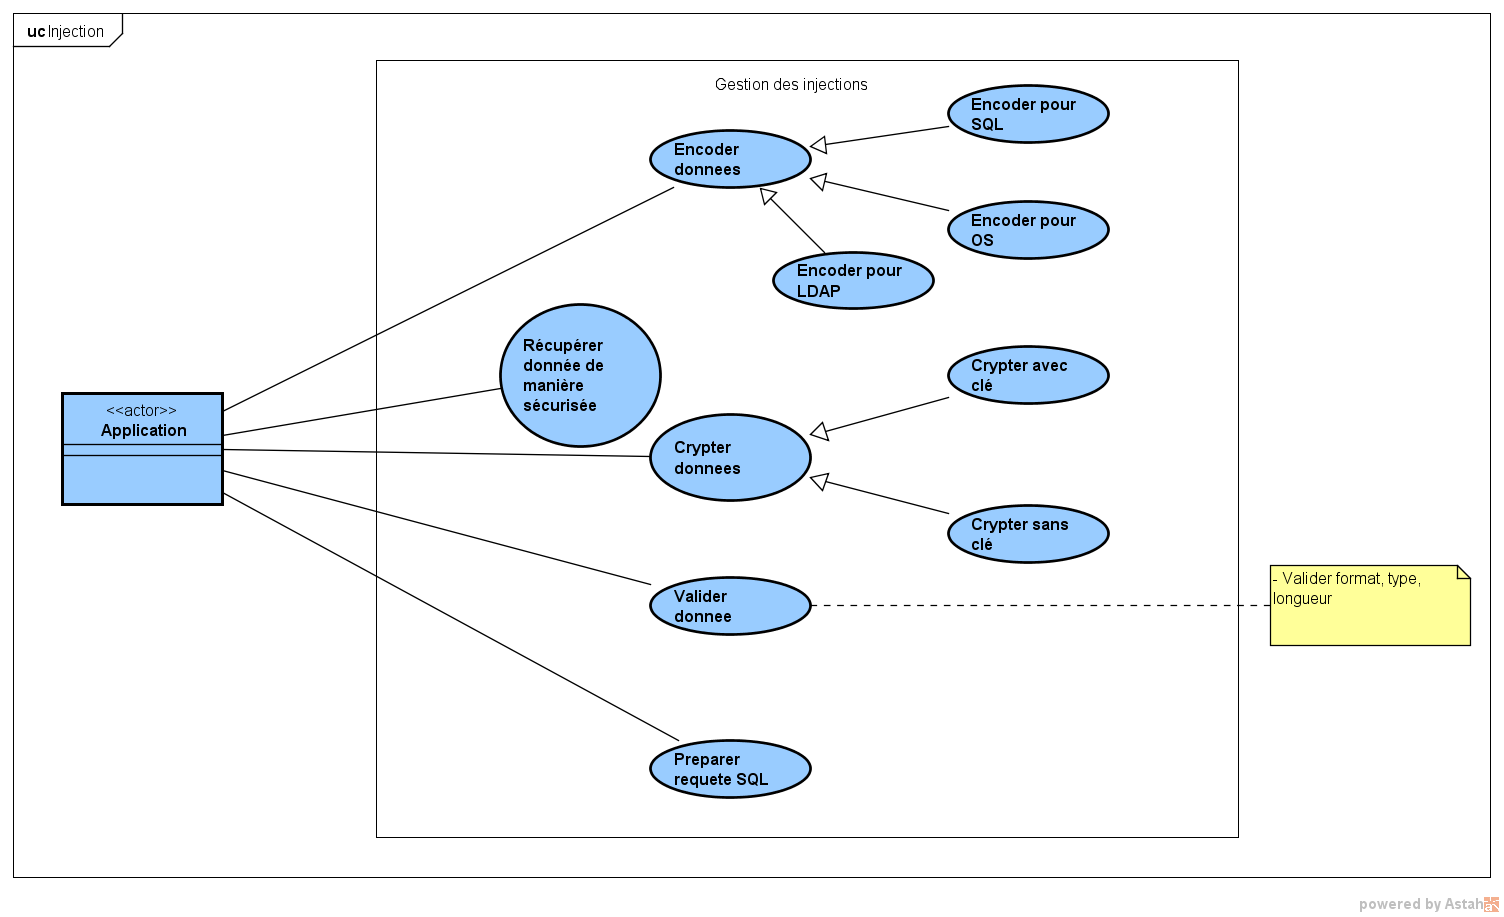
\includegraphics[height=0.27\textheight]{fig/Injection-use-case-diagram.png}}
	\end{minipage}
	\caption{Diagramme de cas d'utilisation du sous-systéme "Gestion des injections"}
	\label{fig:8.1}
\end{figure}

\subsection{Package Gestion des violations de gestion d'authentification}

\subsubsection{Diagramme de cas d'utilisation}
Le diagramme de cas d'utilisation du package "Gestion des violations de gestion d'authentification" est representé ci-dessous. Il comprend les cas d'utilisation permettant à une application donnée de mitiger les risques de violations de gestion d'authentification.\\ 
\begin{figure}[h!]
	\centering
	\begin{minipage}{12cm}
		\centering
		{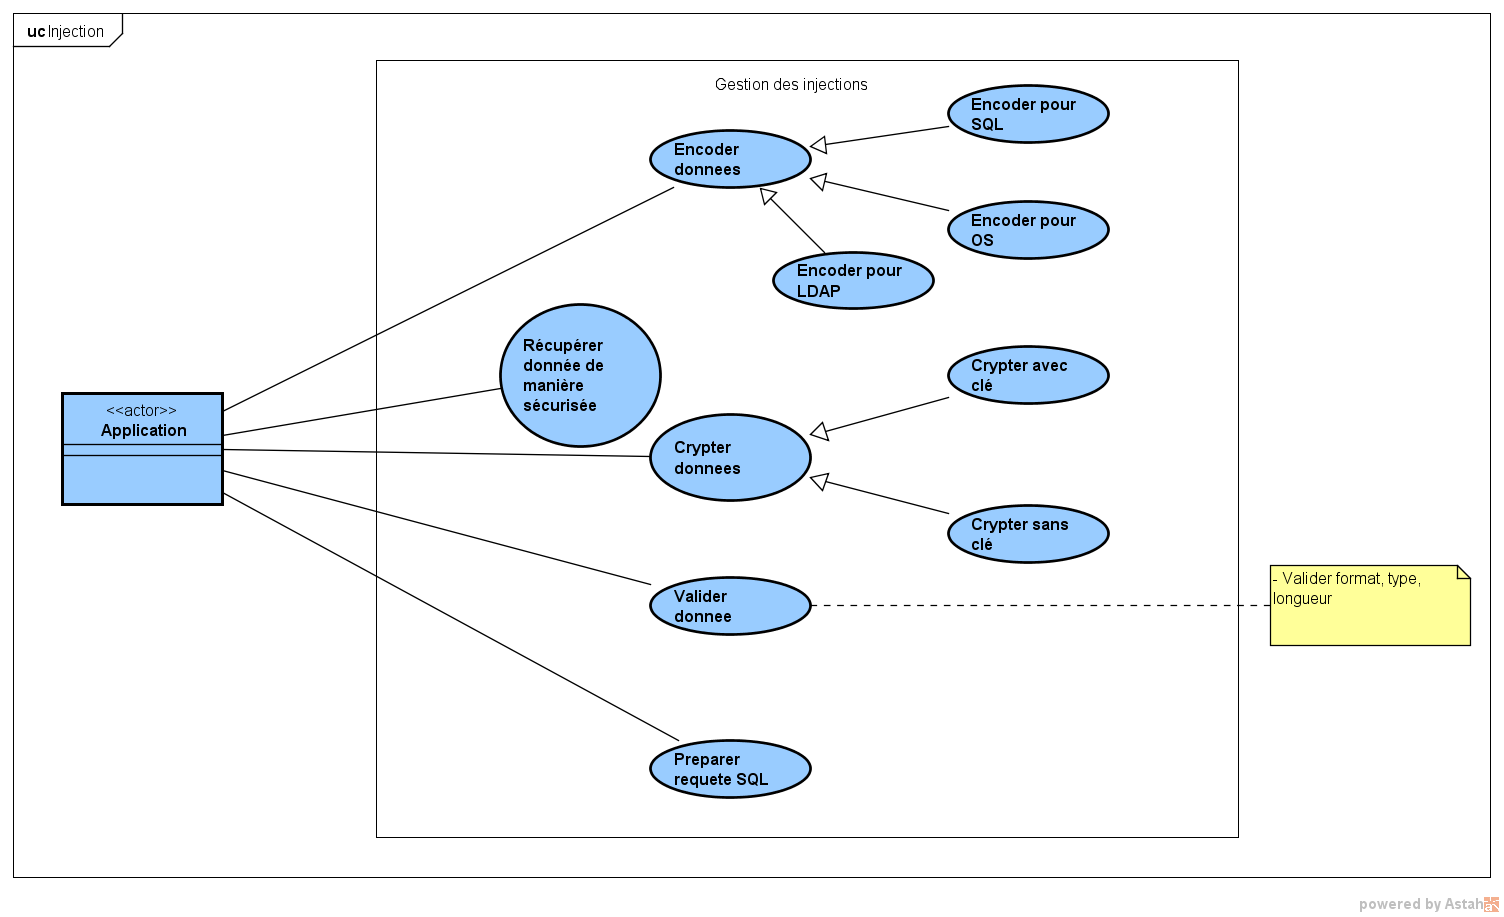
\includegraphics[height=0.27\textheight]{fig/Injection-use-case-diagram.png}}
	\end{minipage}
	\caption{Diagramme de cas d'utilisation du sous-systéme "Gestion des injections"}
	\label{fig:8.1}
\end{figure}

\subsection{Système global}
Both ESAPI and this book are organized around fundamental security controls. We have not created
chapters around common vulnerabilities or attacks, such as XSS, CSRF, SQL injection, etc… Books
organized this way are sexy, but don’t encourage the best architecture possible. \\
For example, if you are trying to stamp out XSS from your enterprise, the right way to do it is to establish great input validation and output encoding mechanisms that developers can use easily. We discuss these two fundamental controls in our book. But those same controls help to stop a wide range of other attacks as well. We believe that focusing on getting the right controls in place is the path to improved software security. 